
    \subsection{The Foundation of the Models}

    To build the models, a set of Python libraries is utilized, mainly PyTorch, NumPy, TensorBoard, and Einops. PyTorch serves as the core tool for constructing and training the models.
    
    The models discussed in this thesis are based on a Python script by A. Karpathy named NanoGPT \autocite{nanoGPTkarpathy2023}. This script demonstrates a straightforward and accessible GPT implementation. 
    
    \subsubsection{Data Handling}
    
    For data management, a script named dataSetCombiner is developed to load and return a combined dataset from specified image folders with optional transformations. The function combines the 33 different sources from multiple directories into a single dataset, also offering the option to apply various image transformations such as cropping, flipping, gray scaling, and color jitter.
    
    It allows for the selection between 512x512 and 1024x1024 pixel datasets, depending on the use case. Parameters can be adjusted to tailor the dataset to specific needs, such as image size, the particular dataset to load, and the option to include multiple instances of the dataset. Furthermore, it can randomly flip images vertically or horizontally to augment the dataset, thereby preventing overfitting and improving model generalization. It also supports color jittering, allowing for random adjustments in image brightness, contrast, saturation, and hue, which introduces further variability into the dataset when needed. Additionally, an option to convert images to grayscale is available.
    

\begin{figure}[H]
\centering
\begin{lstlisting}[language=Python]
    def getDataSet(path, dataset_name, size_x, size_y, repeatData=1, random_vertical_flip=False, random_horizontal_flip=False, crop_type='random', grayscale=False, color_jitter=False, jitter_brightness=0, jitter_contrast=0, jitter_saturation=0, jitter_hue=0):
\end{lstlisting}
\caption{Python function declaration: getDataSet}
\label{fig:getDataSet}
\end{figure}


    \subsubsection{Monitoring Training Progress}
    
    The training process is monitored using TensorBoard, a tool that helps visualize different aspects of training. In this thesis, TensorBoard is particularly useful for tracking training and validation loss through plots. It also allows for the viewing of the input images and the outputs generated by the models.    
    
\newpage


\subsection{Column Image Transformer}
    
    The Column Image Transformer is a transformer-based model that processes input data in a columnar format as examined in detail see \autoref{sec:IntroColumnModel}.
    
    \subsubsection{Get Data as Columns}

    The data is loaded as a DataLoader object, which is then iterated over to obtain the data in (Batch, Color, Height, Width) format. The data is then reshaped into a columnar format, resulting in a tensor of shape (Batch, Height, Color). This reshaping is achieved by indexing the data tensor as follows:

\begin{figure}[H]
\centering
\begin{lstlisting}[language=Python]

# data: (Batch, Color, Height, Width)
def get_batch(data):

    x = data[:, :BLOCK_SIZE, :BATCH_SIZE]
    y = data[:, 1:BLOCK_SIZE+1, :BATCH_SIZE]

    x = rearrange(x, 'c h b -> b h c')
    y = rearrange(y, 'c h b -> b h c')

    return x, y
\end{lstlisting}
\caption{Python function to convert data into a columnar format}
\label{fig:get_batch_CIT}
\end{figure}

    The resulting tensor x is the input to the model, and the tensor y is the target output. The y tensor is shifted by one position to the right so that the model can learn to predict the next column based on the previous columns.

    \subsubsection{Pixel Embedding}

    The input part of the data \(x\) is embedded into a higher-dimensional space using pixel embedding layers. This MLP is a straightforward linear layer that maps the input data to a higher-dimensional space, transitioning from 3 color channels to \(N_{\text{EMBD}}\). This layer consists of a linear transformation followed by a ReLU activation function and is succeeded by a dropout layer.

    Through testing and experimentation, it was discovered that the optimal configuration for the pixel embedding layer involves a specific sequence of dimensionality increases. The most effective pathway identified begins by scaling the dimensionality of the input from the original image channels \(C\) to one-fifth of \(N_{\text{EMBD}}\) (\(\frac{1}{5}N_{\text{EMBD}}\)), then increasing it to one-half of \(N_{\text{EMBD}}\) (\(\frac{1}{2}N_{\text{EMBD}}\)) until reaching \(N_{\text{EMBD}}\). The pixel embedding layer is followed by a dropout layer with a dropout rate of 0.2.

    It is crucial to highlight the importance of excluding a layer normalization (layernorm) layer in the initial few layers of the model. Incorporating layernorm early on results in outputs that are predominantly black and white. This phenomenon occurs because the color channels \(C\), which are comprised of Red, Green, and Blue, are normalized by the layernorm layer to exhibit uniform values across these channels. As a consequence, this normalization process hinders the model's ability to learn the distinct colors of the pixels, relegating it to only wrong grayscale variations.

    \subsubsection{Positional Embedding}

    \subsubsection{Classification or Regression}

    \subsubsection{Discriminator}

\newpage


\subsection{Spiral Image Transformer}
    (explanation, Data to Spiral form, positional embedding, )

    As explained in the previous section (see Section \ref{sec:IntroSpiralModel}), the spiral model is a transformer-based model that employs a spiral architecture to process input data. 

    \subsubsection{Spiral}

    To convert the 3-dimensional data (color channels, image height, image width) into a spiral form, the data must be unrolled into one dimension, resulting in an output format of (color channels, spiral length). Consequently, the data width and the height dimensions must be squeezed into a single dimension. This new form can then be utilized similarly to the data in the Column Image Transformer. As the data is flattened into a single dimension, it allows for an easy addition of positional embedding.

    \subsubsection{Spiral generation}

    The conversion of data into a spiral form needs to be highly efficient because the code block will execute for every image (batch) in the dataset. Therefore, a simple nested for loop is insufficient. In this example, fancy indexing is used to convert the data into a spiral form. Thus, the data tensor is indexed with a two-dimensional tensor containing the indices of the spiral form.

    At the start of the model training script, one indexing spiral is created to be used for all images in the dataset. The following code block illustrates the creation of the spiral index tensor.

\begin{figure}[H]
\centering
\begin{lstlisting}[language=Python]
def create_spiral(n): # n = width and height
    
    matrix = [[0] * n for _ in range(n)] # Initialize n x n matrix

    x, y = 0, 0
    # Direction vectors (right, down, left, up)
    dx = [0, 1, 0, -1]
    dy = [1, 0, -1, 0]
    direction = 0

    for i in range(n * n - 1, -1, -1):  # Start (35 for 6x6)
        matrix[x][y] = i
        nx = x + dx[direction]
        ny = y + dy[direction]

        # Change direction if the next position: out of bounds or filled
        if nx<0 or nx>=n or ny<0 or ny>=n or matrix[nx][ny]!=0:
            direction = (direction + 1) % 4  # Change direction
            nx = x + dx[direction]
            ny = y + dy[direction]

        x, y = nx, ny
    
    return torch.tensor(matrix)
\end{lstlisting}
\caption{Python function to create a spiral index tensor}
\label{fig:spiral_matrix}
\end{figure}

    The code above generates a square matrix of size n by n, then fills it with numbers in a spiral pattern, starting from the outer edge and spiraling inwards clockwise. Each cell of the matrix is assigned a unique number, beginning from the highest value in the top-left corner and decreasing by one with each step along the spiral path until reaching zero at the center or the end of the spiral. The spiral formation is achieved by moving right, then down, then left, then up, and repeating this sequence, adjusting direction whenever the next step would go out of bounds or into a cell that's already been filled.


    \subsection{Fancy Indexing into the Spiral form}

    The spiral index tensor is then used to index the data tensor, effectively converting it into a spiral form. The following image illustrates the process of converting a 7x7 image.
    
    
    \begin{figure}[H]
    \centering
    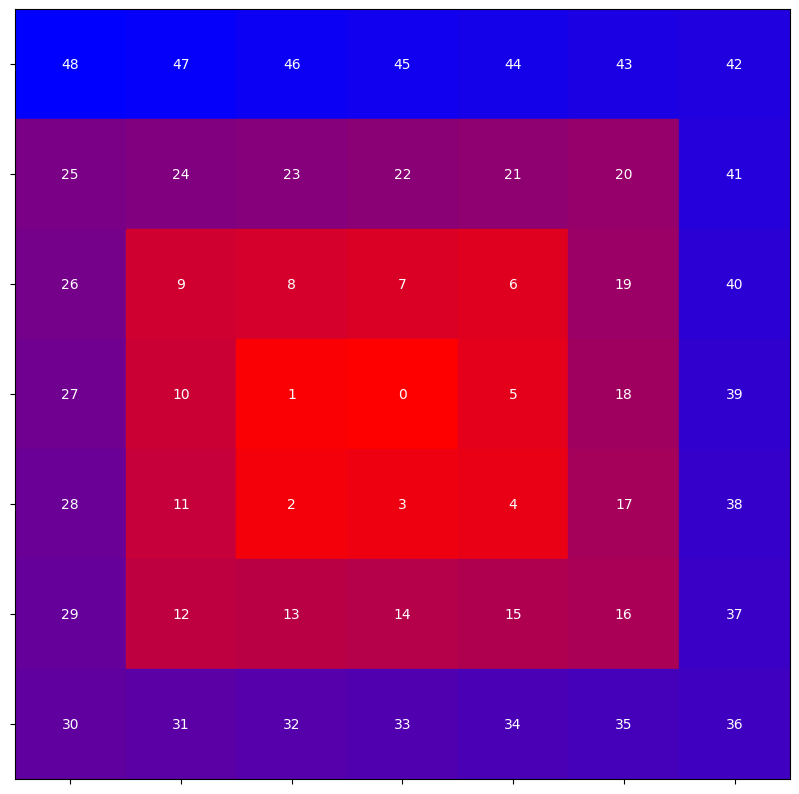
\includegraphics[width=0.6\textwidth]{../code/dataAnalysis/plots/exampleImgs/spiralShowcase1.png}
    \caption{Image representation}
    \label{fig:spiral_indexing_1}        
    \end{figure}

    \begin{figure}[H]
    \centering
    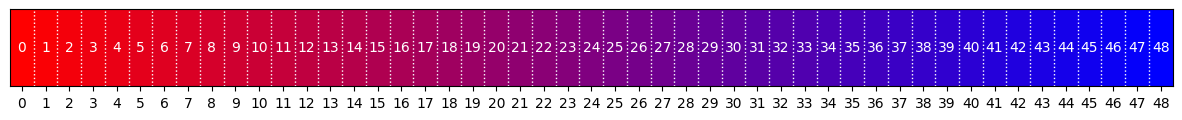
\includegraphics[width=1\textwidth]{../code/dataAnalysis/plots/exampleImgs/spiralShowcase0.png}
    \caption{7x7 Image flattened into a spiral form} 
    \label{fig:spiral_indexing_0}        
    \end{figure}

    As you can see in \autoref{fig:spiral_indexing_1}, the pixels of the image are labeled with their respective indices 0, \dots, 43. The image is then unrolled into a single dimension, as shown in \autoref{fig:spiral_indexing_0}. The centering pixel is the first element of the spiral, and the spiral continues counterclockwise from there. In the model script, the dimensions for width and height typically exceed 7, yet the underlying process remains unchanged.

\begin{figure}[H]
\centering
\begin{lstlisting}[language=Python]
  spiral_indices = torch.tensor(create_spiral(IMAGE_SIZE))

  # [...]
  # Batch_size, Color_channels, Height, Width
  B, C, H, W = data.shape

  spiral_data = torch.zeros_like(data.view(B, C, -1))

  spiral_data[:,:,spiral_indices.flatten()] = data.view(B, C, -1)

  # [...]
\end{lstlisting}
\caption{Fancy indexing to convert data into a spiral form}
\label{fig:spiral_indexing_code}
\end{figure}

    \subsubsection{Positional embedding}

\subsection{Problems}
    (layer norm(sigmoid vs clamp), color shift to gray (illustrations of average color), Text tokens vs imgs tokens)